\documentclass[a4paper]{article}
\usepackage[14pt]{extsizes} % для того чтобы задать нестандартный 14-ый размер шрифта
\usepackage{amsmath}
\usepackage[unicode, pdftex]{hyperref} % гиперссылки
\usepackage[usenames]{color} %цвета
\usepackage{mathtext}
\usepackage[T2A]{fontenc}
\usepackage[utf8]{inputenc}
\usepackage[english, russian]{babel}
\usepackage{amsfonts}
\usepackage{float} % для нормального расположения картинок и таблиц
\usepackage[left=20mm, top=15mm, right=15mm, bottom=15mm, nohead, footskip=10mm]{geometry} % настройки полей документа
\usepackage{graphicx} % работа с картинками 
\usepackage{wrapfig}
\usepackage{placeins} % работа с картинками (их корректная вставка в текст)
\usepackage{misccorr} % в заголовках появляется точка, но при ссылке на них ее нет
\usepackage{indentfirst} % красная строка у первой строки раздела
\DeclareMathSymbol{,}{\mathord}{letters}{"3B} % убирает пробел после запятой в формулах
%% Определяем свой шрифт "lsumb"
\DeclareSymbolFont{lsymb}{U}{euex}{m}{n}
%% Определяем интегралы
\DeclareMathSymbol{\intop}{\mathop}{lsymb}{"52}
\DeclareMathSymbol{\ointop}{\mathop}{lsymb}{"48}
\DeclareMathSymbol{\smallint}{\mathop}{lsymb}{"52}
%Красивая ЭДС с завитушками
\usepackage{mathrsfs}
\DeclareSymbolFont{rsfs}{U}{rsfs}{m}{n} \DeclareSymbolFontAlphabet{\mathscr}{rsfs}
\DeclareMathSymbol{\EDS}{\mathord}{rsfs}{`E}
\usepackage{amssymb} %русские неравенства: \leqslant \geqslant
%Пакет дял таблиц   
\usepackage{multirow}
%\usepackage{subcaption,floatrow,graphicx,calc}

\usepackage{hhline}
\usepackage{diagbox}
\usepackage{array}
\usepackage{float}



 % Ссылки?
\usepackage{hyperref}
\usepackage[rgb]{xcolor}
\hypersetup{				% Гиперссылки
    colorlinks=true,       	% false: ссылки в рамках
	urlcolor=blue          % на URL
}


\begin{document}% начало документа
% НАЧАЛО ТИТУЛЬНОГО ЛИСТА
\begin{center}
	\hfill \break
	\hfill \break
	{\small ФЕДЕРАЛЬНОЕ ГОСУДАРСТВЕННОЕ АВТОНОМНОЕ ОБРАЗОВАТЕЛЬНОЕ\\ УЧРЕЖДЕНИЕ ВЫСШЕГО ОБРАЗОВАНИЯ\\ МОСКОВСКИЙ ФИЗИКО-ТЕХНИЧЕСКИЙ ИНСТИТУТ\\ (НАЦИОНАЛЬНЫЙ ИССЛЕДОВАТЕЛЬСКИЙ УНИВЕРСИТЕТ)\\ ФАКУЛЬТЕТ ОБЩЕЙ И ПРИКЛАДНОЙ ФИЗИКИ}\\
	\hfill \break
	\hfill \break
	\hfill \break
	\hfill \break
	\hfill \break
	\normalsize{ЛАБОРАТОРНАЯ РАБОТА ПО ФИЗИКЕ}\\
	\hfill \break
	\hfill \break
	\hfill \break
	\hfill \break
	\normalsize{\textbf{Работа № 3.4.2}}\\
	\hfill \break

	\hfill \break
	\large{<<Закон Кюри-Вейсса>>}\\
\end{center}
\hfill \break
\hfill \break
\hfill \break
\hfill \break



\begin{flushright}
	\normalsize{Студента 2 курса группы Б02-005}\\
	\normalsize{\textbf{Гусарова Николая}}\\
\end{flushright}
\hfill \break
\hfill \break
	\hfill \break
	\hfill \break
	\hfill \break
	\hfill \break
\hfill \break
\hfill \break
\hfill \break
\hfill \break

\begin{center}
	\normalsize{\textbf{Долгопрудный, Ноябрь 2021}}
\end{center}


\thispagestyle{empty} % выключаем отображение номера для этой страницы

% КОНЕЦ ТИТУЛЬНОГО ЛИСТА

	
	\newpage
	\section{Аннотация}
    \textbf{Цель работы}: изучение температурной зависимости магнитной восприимчивости ферромагнетика выше точки Кюри.\\
    
	
	\textbf{В работе используется:}катушка самоиндукции с образцом из гадолиния, термостат, частотомер, цифровой вольтметр, LC-автогенератор, термопара медь-константан.\\
	
	\section{Теоретическая часть}	 
	 \subsection{Магнитное поле в веществе}	 
	Известно, что вещество может обладать как собственной намагниченностью, так и изменять свою намагниченность при помещении во внешнее магнитное поле. Микроскопическими источниками магнитного поля в среде являются орбитальное движение электронов в молекулах и атомах, а также собственное вращение (спин) электронов и ядер. При макроскопическом описании свойств среды можно считать, что каждый элемент объёма среды может являться элементарным источником магнитного поля --- магнитным диполем. Для описания усреднённых свойств
среды используют \textbf{вектор намагниченности $\vec{M}$}, равный магнитному моменту единичного объёма вещества (объёмная плотность магнитного момента, размерность в системе СИ $ [M] = \dfrac{A \cdot m^2}{m^3} =  \dfrac{A}{m}$).\\

Магнитное поле на микроскопическом уровне (на масштабах атомов) $B_{\text{микро}}$ испытывает резкие изменения в пространстве. Величина магнитного поля $B$ в данной точке среды определяется как значение микрополя, усреднённое по малому (элементарному) объёму, содержащему при этом большое количество частиц: 
 $\vec{B}= \lim\limits_{\Delta V \to 0} \iiint\limits_{\Delta V } \vec{B_{\text{микро}}} dV$.
Вектор $\vec{B}$ называют \textbf{индукцией поля} (размерность $ [B] = \dfrac{H}{m\cdot A} \equiv Тл$).\\

Помимо этого, $\vec{H}$ называется \text{напряжённостью поля}, размерность в системе СИ $ [H] =  \dfrac{A}{m}$, опрееляемый из соотношения:\\
$\vec{B} = \mu_{0}(\vec{H}+\vec{M})$, где  $\mu_{0} = 4\pi \cdot 10^{-7} \dfrac{H}{A^2}$ магнитная постоянная \\

В простейшем практически важном случае намагниченность $\vec{M}$ в каждой точке среды прямо пропорциональна вектору напряжённости магнитного поля $\vec{H}$ в этой же точке
\begin{equation}\label{1}
\vec{M} = \chi \vec{H}.
\end{equation}

Коэффициент $\chi$ называют \textbf{магнитной восприимчивостью} среды. Вещества, для которых закон (1) выполняется с хорошей точностью, называют  \textbf{парамагнетиками} ($\chi > 0$) и  \textbf{диамагнетиками} ($\chi < 0$). В парамагнетиках элементарные диполи ориентированы в основном по приложенному полю, а в диамагнетиках — против него.\\

Если закон (1) применим, то можно записать
\begin{equation}\label{2}
\vec{B} = \mu \mu_0 \vec{H},
\end{equation}
где $\mu = 1+\chi$ --- \textbf{магнитопроницаемость} вещества.\\
В системе СГС имеют место соотношения:\\
$\vec{B} = \vec{H}+4\pi \vec{M} = \mu \vec{H}$, $\mu  = 1+4\pi \chi$\\
 В общем случае зависимость $M(H)$ может быть нелинейной, а также зависеть от «предыстории» образца, то есть значений полей в предыдущие моменты времени — явление \textbf{гистерезиса} в ферромагнетиках.
	
	
	\subsubsection{Свойства магнитных сред. Парамагнетизм}
	Парамагнетизм ($\chi > 0$) характерен для веществ, микроскопические частицы которых (атомы, ионы, молекулы) обладают собственным магнитным моментом в отсутствие внешнего магнитного поля. В парамагнетиках энергия взаимодействия между соседними магнитными моментами атомов мала по сравнению с тепловой энергией, поэтому в отсутствие внешнего магнитного поля микроскопические магнитные моменты полностью разупорядочены, и намагниченность среды равна нулю. При помещении во внешнее поле магнитным моментам энергетически выгодно ориентироваться преимущественно по полю, что и приводит к парамагнитному эффекту.\\
Оценим температурную зависимость магнитной восприимчивости парамагнетика в классической модели. Пусть среднее число атомов в еди­нице объёма равно \textbf{$n$}, а абсолютная величина магнитного момента атома \textbf{$m_a$}. В магнитном поле с индукцией $B$ энергия магнитного диполя, составляющего с направлением поля угол $\alpha$, равна\\
$U = -\textbf{$m_a$}B \cos{\alpha}$\\
и может меняться в диапазоне от $-\textbf{$m_a$}B$ до $+\textbf{$m_a$}B$.\\
Из термодинамики известно, что доля атомов $dn$, обладающих в условиях равновесия энергией $U(\alpha)$, определяется распределением Больцмана:\\
\begin{equation}\label{}
dn  \propto e^{-\dfrac{U(\alpha)}{k_{\text{Б}}T}} d \alpha 
\end{equation}
Пусть внешнее магнитное поле достаточно мало, так что энергия магнитных моментов атомов в нём много меньше тепловой:  $m_aB$ много меньше $k_{\text{Б}}T$. Число атомов, имеющих положительную ($\alpha > 0$) проекцию на направление $B$, может быть записано как(воспользовались разложением экспоненты от малого параметра):\\
\begin{equation}\label{}
n_{\text{+}}  = n_0 e^{\dfrac{m_aB}{k_{\text{Б}}T}} \approx n_0 (1+\dfrac{m_aB}{k_{\text{Б}}T})
\end{equation}
Для атомов с отрицательной проекцией момента ($\alpha < 0$):
\begin{equation}\label{}
n_{\text{---}}  = n_0 e^{-\dfrac{m_aB}{k_{\text{Б}}T}} \approx n_0 (1-\dfrac{m_aB}{k_{\text{Б}}T})
\end{equation}
Из условия нормировки $n = n_{\text{---}}+n_{\text{+}}$\\
Величину суммарного магнитного момента единицы объёма можно оценить как\\
$M \sim n_{\text{---}}\cdot(-m_a) +n_{\text{+}}\cdot m_a \approx \dfrac{n m_a^2}{k_{\text{Б}}T}B$\\
Более аккуратное усреднение по углам даст поправочный множитель
порядка единицы (в классической модели получается коэффициент 1/3).
Таким образом, парамагнитная восприимчивость равна
\begin{equation}\label{3}
\chi_{\text{пар}} \sim  \propto \dfrac{1}{T}\\
\end{equation}
Температурная зависимость восприимчивости парамагнетиков вида (6) называется \textbf{законом Кюри}.

	\subsubsection{Ферромагнетизм}
	 Cуществуют вещества, способные сильно намагничиваться даже в небольших полях. Такие вещества относят к классу \textbf{ферромагнетиков}. Это — железо, никель, кобальт, гадолиний и их многочисленные сплавы. Ферромагнитными свойствами обладают некоторые сплавы элементов, которые порознь не являются ферромагнитными (например, сплавы меди и марганца), и ряд неметаллических веществ (ферриты). 
Зависимость намагниченности от напряжённости магнитного поля у всех ферромагнетиков оказывается нелинейной $M(H)$: магнитная восприимчивость $\chi$ не является константой и $\chi(H)$. По абсолютной величине восприимчивость достигает значений $10^3 - 10^4$
(ср. с парамагнетиками, для которых  $\chi \sim 10^{-7} - 10^{-5}$). Кроме того, анизотропия кристаллической решётки приводит к тому, что $\chi$ может иметьтензорный характер (векторы M и H не сонаправлены).\\
Как и в случае парамагнетиков, атомы ферромагнетика обладают собственным магнитным моментом. Однако даже в отсутствие внешнего магнитного поля атомы ферромагнетика способны образовывать упорядоченные структуры (\textbf{домены}), в которых все магнитные моменты ориентированы практически в одном направлении. Таким образом, каждый отдельный атом испытывает влияние не только внешнего поля, но и поля, созданного коллективом его соседей.\\
	\textbf{Образование доменов.}\\
	Остановимся кратко на причине, по которой соседним магнитным моментам выгодно объединяться в домены.
В первую очередь, магнитное (диполь-дипольное) взаимодействие между атомами не может привести к упорядочению системы. \\
        \begin{figure}[H]
		\centering
		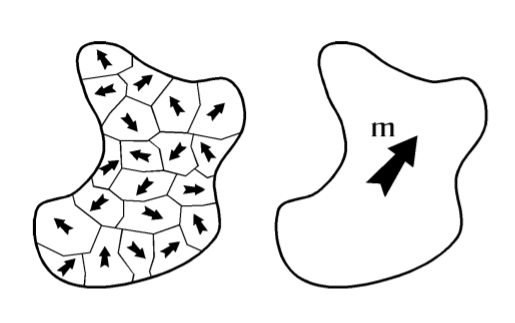
\includegraphics[width=6cm]{theory1.png}
		\caption{Доменная структура ферромагнетика при слабом и сильном внешнем поле}
	\end{figure} 
Единственное взаимодействие, которое способно выстроить в ряд магнитные моменты электронов в атомах при температурах порядка комнатной, --- это электростатическое взаимодействие (порядка 1 эВ). Как следует
из квантовой механики, если магнитные моменты (или спины) электронов соседних атомов сонаправлены, их электростатическое отталкивание становится меньше. Таким образом, магнитным моментам атомов энергетически выгодно ориентироваться в одном направлении. Такое явление получило название \textbf{обменного взаимодействия}.
	\textbf{Модель среднего поля.}\\
	В качестве простейшей эмпирической модели, описывающей такую ситуацию, можно рассмотреть следующую модель: предположим, что намагниченность элемента среды пропорциональна некоторому эффективному полю $H_{ef}$, складывающемуся из поля $H$ в данной точке, созданного сторонними токами, и среднего «коллективного» поля, пропорционального величине намагниченности $M$:
\begin{equation}\label{}
\vec{M} = \chi_{\text{пар}} \vec{H_{ef}},  \vec{H_{ef}} = \vec{H}+\beta \vec{M}
\end{equation}
где $\chi_{\text{пар}}$ — парамагнитная восприимчивость отдельного атома (6), $\beta$ --- некоторая безразмерная константа, определяемая из опыта.
Модель среднего поля позволяет уточнить закон Кюри:
\begin{equation}\label{}
\chi \propto \dfrac{1}{T-\Theta}
\end{equation}
где параметр $\Theta = \beta \mu_0 \dfrac{n m_a^2}{3k_{\text{Б}}T}B$ имеет размерность температуры.\\
Соотношение называют \textbf{законом Кюри-Вейсса}. \\
Существует температура $\Theta_K$, называемая \textbf{точкой кюри}, в которой имеет место фазовый
переход (2-го рода) между парамагнитным (при $T>\Theta_K$) и ферромагнитным (при $T<\Theta_K$) состояниями среды. Закон Кюри–Вейсса удовлетворительно выполняется вдали от $\Theta_K$, однако нарушается при приближении к точке перехода, где модель среднего поля становится
слишком груба. Поэтому параметр $\Theta$ несколько отличается от
температуры Кюри: как правило, $\Theta_K < \Theta$.

\subsubsection{Закон Кюри-Вейса}
Вещества с отличными от нуля атомными магнитными моментами
обладают парамагнитными свойствами. Внешнее магнитное поле ориентирует магнитные моменты, которые в отсутствие поля располагались
в пространстве хаотичным образом. При повышении температуры T возрастает дезориентирующее действие теплового движения частиц, и магнитная восприимчивость парамагнетиков убывает по закону Кюри --- обратно пропорционально температуре.\\
Температуру фазового перехода парамагнетик–ферромагнетик называют температурой Кюри $\Theta_K$. Температурная зависимость магнитной восприимчивости у ферромагнетиков выше точки Кюри с удовлетворительной
точностью описывается законом Кюри-Вейсса .
Непосредственно вблизи $\Theta_K$ закон Кюри–Вейсса нарушается. На практике наблюдается зависимость.

\subsubsection{Из условий экспериментальной установки}
Коэффициент самоиндукции катушки $L$ пропорционален магнитной проницаемости $\mu$ заполняющей его среды: $L \propto \mu$. Тогда разность самоиндукций катушки с образцом $L$ и без него $L_0$ будет пропорциональна восприимчивости образца $\chi$:
\begin{equation}\label{}
L-L_0 \propto \mu - 1 = \chi.
\end{equation}
При изменении индуктивности образца меняется период колебаний автогенератора:
\begin{equation}\label{}
\tau = 2\pi \sqrt{LC}
\end{equation}
где C --- ёмкость контура автогенератора. Период колебаний в отсутствие образца определяется самоиндукцией пустой катушки:
\begin{equation}\label{}
\tau_0 = 2\pi \sqrt{L_0 C}
\end{equation}
Отсюда находим
\begin{equation}\label{}
\chi \propto L-L_0 \propto \tau^2 - \tau_0^2
\end{equation}
Из формул следует, что закон Кюри–Вейсса справедлив, если выполнено соотношение:
\begin{equation}\label{}
\dfrac{1}{\tau^2  - \tau_0^2} \propto T - \Theta_p
\end{equation}


	\subsection{Экспериментальная установка}
	В работе изучается температурная зависимость $\chi(T)$ гадолиния при температурах выше точки Кюри. Исследуемый ферромагнитный образец (гадолиний) расположен внутри пустотелой катушки самоиндукции, которая служит индуктивностью колебательного контура, входящего в состав LC-автогенератора(генератора колебаний с самовозбуждением). \\
	 Масло предохраняет образец от окисления и способствует ухудшению электрического контакта между отдельными частичками образца.
        \begin{figure}[H]
		\centering
		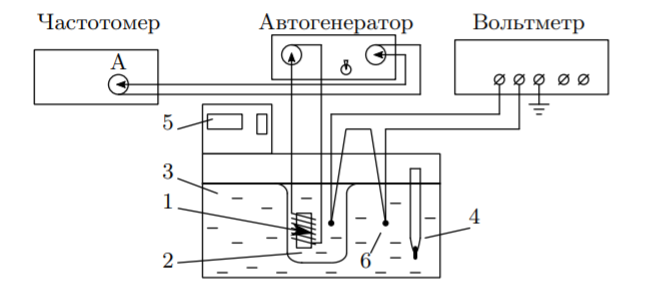
\includegraphics[width=13cm]{theory2.png}
		\caption{Схема экспериментальной установки}
	\end{figure}  

	
	
	\section{Измерения и обработка результатов}

	
    \subsection{Проведение измерений}
\begin{table}[H]
    \centering
    \caption{Зависимость периода колебаний LC- генератора от температуры образца, без учёта значений с термопары}
    \begin{tabular}{|l|l|l|}
    \hline
    $t, ^\circ C$ & $\tau, us$ & $\Delta U, mV$\\\hline
        10,17 & 10,864 & -0,001 \\ \hline
        12,11 & 10,833 & -0,008 \\ \hline
        14,12 & 10,770 & -0,006 \\ \hline
        16,11 & 10,666 & -0,006 \\ \hline
        18,12 & 10,485 & -0,004 \\ \hline
        20,11 & 10,213 & -0,008 \\ \hline
        22,09 & 9,836 & -0,008 \\ \hline
        24,10 & 9,539 & -0,008 \\ \hline
        26,10 & 9,402 & -0,008 \\ \hline
        28,11 & 9,325 & -0,005 \\ \hline
        30,09 & 9,280 & -0,007 \\ \hline
        32,10 & 9,246 & -0,005 \\ \hline
        34,09 & 9,224 & -0,009 \\ \hline
        36,08 & 9,205 & -0,008 \\ \hline
        38,08 & 9,191 & -0,009 \\ \hline
        40,07 & 9,180 & -0,010 \\ \hline
    \end{tabular}
\end{table}
    
    \subsection{Обработка результатов}
Рассчитаем температуру $T$ образца с учётом показаний термопары с чувствительностью $24\dfrac{degree}{mV}$. Измерения проводились, когда разность температур была меньше 0,25К, то есть $|\Delta U|< 0.01mV$.
Результаты приведены в таблице2, 
\begin{table}[H]
    \centering
    \caption{Зависимость $f(T)$}
    \begin{tabular}{|l|l|}
    \hline
        T, K & $\tau, us$ \\ \hline
        283,30 & 10,86 \\ \hline
        285,07 & 10,83 \\ \hline
        287,13 & 10,77 \\ \hline
        289,12 & 10,67 \\ \hline
        291,17 & 10,49 \\ \hline
        293,07 & 10,21 \\ \hline
        295,05 & 9,84 \\ \hline
        297,06 & 9,54 \\ \hline
        299,06 & 9,40 \\ \hline
        301,14 & 9,33 \\ \hline
        303,07 & 9,28 \\ \hline
        305,13 & 9,25 \\ \hline
        307,02 & 9,22 \\ \hline
        309,04 & 9,21 \\ \hline
        311,01 & 9,19 \\ \hline
        312,98 & 9,18 \\ \hline
    \end{tabular}
\end{table}


Построим график зависимости $f(T) = \dfrac{1}{\tau^2 - \tau_0^2}$. Используя МНК и экстраполируя полученную прямую(значения температур выше 297К) к оси абсцисс, определим парамагнитную точку Кюри $\Theta_p$ для гадолиния.
        \begin{figure}[H]
		\centering
		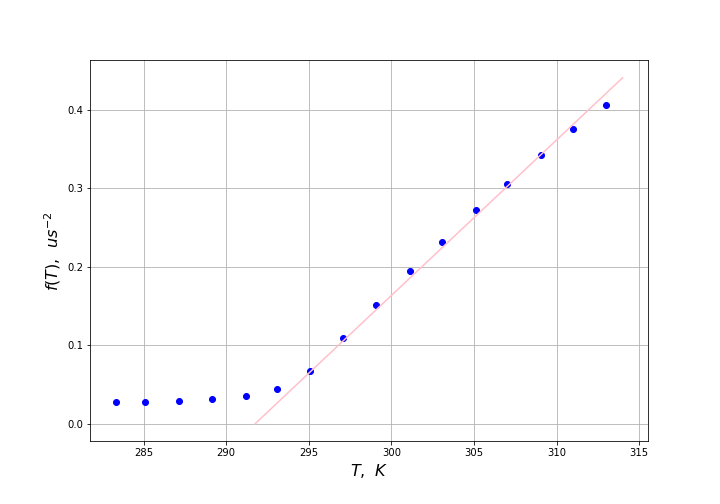
\includegraphics[width=13cm]{plot1.png}
		\caption{Зависимость $f(T) = \dfrac{1}{\tau^2 - \tau_0^2}$}
	\end{figure}  
Получили прямую вида $y= kx+b$, где:
\begin{equation}\label{}
f(T) = (187 \pm 3) \cdot 10^{-4} \dfrac{1}{K\cdot us^2} T - (5.4 \pm 0.1)\dfrac{1}{us^2}
\end{equation}
отсюда получаем, что $\Theta_p = (291 \pm 2)K$

Непосредственно вблизи точки Кюри закон Кюри-Вейса(прямая линия) нарушается. по нашим данным $\Theta_K \approx 295K$.


    
 

\section{Вывод}
Точка Кюри для гадоллиния 292K. В рзультате эксперимента получили  295K. Исследовали поведение гадоллиния(зависимость Кюри-Вейсса при температуре выше, чем температура Кюри), убедились в наличие перехода между свойствами парамагнетика и ферромагнетика.
      
	\end{document}